\section{Zielsetzung}
Ziel des Versuches ist die Untersuchung mehrerer Materialzusammensetzungen von Würfeln, mithilfe von Tomographie mit Gammastrahlung.

\section{Theoretische Grundlagen}

\subsection{Caesium als Gammastrahler}
Unter dem Begriff Gammastrahlung $\gamma$ ist im Allgemeinen eine elektromagnetische Strahlung mit Energien über $\SI{200}{\kilo\electronvolt}$ gemeint. 
Die Wechselwirkungsmöglichkeiten dieser Strahlung mit Materie werden im Folgenden diskutiert. Als Strahlungsquelle bieten sich einige Möglichkeiten, wie hochenergetische Röntgenröhren, oder radioaktive Isotope, an. 
In diesem Fall wird Caesium 137 (\ce{^{137}_{55}Cs}) verwendet. Das Zerfallsschema einer \ce{^{137}_{55}Cs}-Quelle ist dabei in Abbildung \ref{fig:decay} aufgezeigt.
\begin{figure}
    \centering
    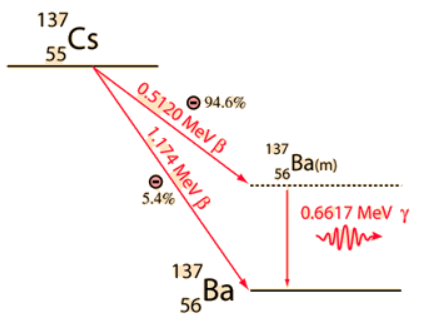
\includegraphics[width=0.5\textwidth]{bilder/decay.png}
    \caption{Zerfallsschema von Caesium 137 nach \cite{decay}.}
    \label{fig:decay}
\end{figure}
Zu erkennen ist ein anfänglicher $\beta^{-}$-Zerfall in einen Bariumzustand. 
Diese beiden Prozesse mitteln sich zu einer Halbwertszeit von $\tau_{1\text{/}2} = 30.07 \text{ Jahren}$. Der deutlich wahrscheinlichere Zerfall geht über einen angeregten Bariumzustand \ce{^{137m}_{56}Ba}. 
Dieser fällt jedoch mit einer kurzen Halbwertszeit von $\tau_{1\text{/}2} = \SI{153}{\second}$ in den stabilen Bariumzustand und gibt dabei eine charakterische Gammastrahlung ab. 
Diese Energie von $E = \SI{661.7}{\kilo\electronvolt}$ stellt den Peak des Energiespektrums von \ce{^{137}_{55}Cs} dar. Aufgrund der langen Halbwertszeit von \ce{^{137}_{55}Cs} handelt es sich um einen Dauerstrahler.
\subsection{Wechselwirkung von Gammastrahlung mit Materie}
Wenn Strahlung jeglicher Art auf ein Medium einfällt, gibt es viele wichtige Faktoren, die die Wechselwirkung mit dem Stoff bestimmen. 
Ein wichtiger Faktor stellt die Art von Strahlung dar. Oft wird hier zu erst zwischen direkt und indirekt ionisierender Strahlung unterschieden. 
Dies liegt vor allem an der Ähnlichkeit ihrer Wechselwirkungsprozesse. Neutronen zeigen eine Ähnlichkeit zu elektromagnetischer Strahlung, da sie beide keine Ladung tragen. 
Außerdem kommt es vor allem bei der Elektronenstrahlung zu weiteren Prozessen wie der Bremsstrahlung. Diese spielt bei der Photonenstrahlung nur eine sekundäre Rolle, da sie erst durch Sekundärelektronen aufkommen kann. 
In unserem Fall wird Gammastrahlung mit einem Intensitätsmaximum von $E = \SI{662}{\kilo\electronvolt}$ betrachtet. 
Die möglichen Wechselwirkungen sind hier bereits stark durch den Energiebereich und die Strahlungsart beschränkt.
Die drei wichtigsten Wechselwirkungsprozesse sind, der Photoelektrsiche Effekt, der Compton-Effekt, sowie die Paarbildung. Diese sind im Folgenden genauer beschrieben.
\subsubsection{Photoeffekt}

\begin{figure}
\begin{minipage}{0.5\textwidth}
Der Photoeffekt beschreibt den Prozess, ein Elektron mithilfe eines Photons aus einem Atom herauszulösen, oder sein Energieniveau anzuregen. 
Er kann immer dann vorkommen, wenn die elektromagnetische Strahlung hinreichend Energie $h\nu_{\text{min}}$ besitzt, um ein Elektron aus seiner Bindung vom Atom zu lösen, oder sein Energieniveau anzuheben. 
Diese Bindungsenergie ist eine sehr spezifische Energie des jeweiligen Atoms. Die nötige Energie zum Herauslösen wird als Austrittsarbeit $W_a$ bezeichnet. 
Der Wirkungsquerschnitt gibt die Wahrscheinlichkeit für das Auftreten des betrachteten Prozesses an.
Da Gammastrahlung bereits eine im klassischen Vergleich große Energie darstellt, kann eine Näherung für große Energien des Wirkungsquerschnittes vorgenommen werden und es zeigt sich
\end{minipage}
\begin{minipage}{0.5\textwidth}
    \centering
    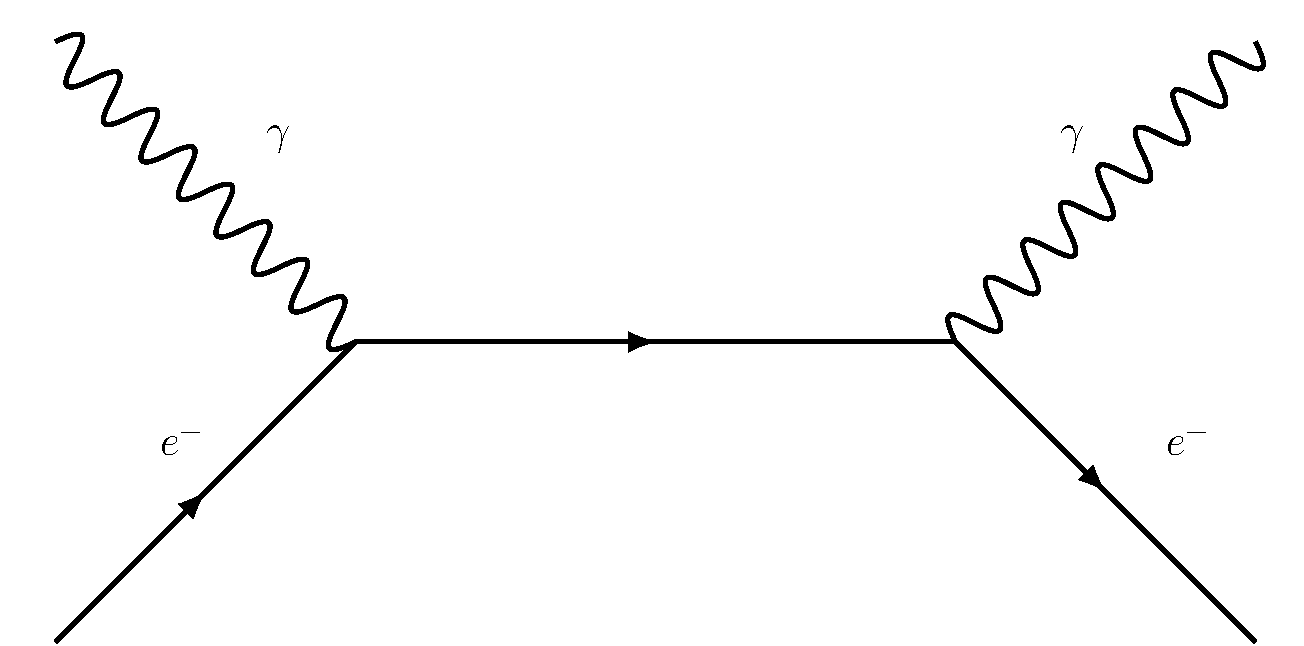
\includegraphics[width=0.9\textwidth]{bilder/compton.pdf}
    \caption{Photo-Effekt. \cite{feynman}}
    \label{fig:hierhier}
\end{minipage}
\end{figure}

\begin{equation*}
\sigma^{\text{Photo}} \propto \frac{Z^{4-5}}{E} \quad | \quad \text{für hohe Energien}.
\end{equation*}
Dabei entspricht $Z$ der Kernladungszahl des Absorbermaterials. 
Die Wahrscheinlichkeit für den Photoeffekt nimmt also mit steigender Photonenenergie ab, es zeigt sich allerdings, dass in den meisten Fällen erst bei Energien einiger Megaelektronenvolt, der Compton-Effekt stark dominiert. 
Ein Abbild des Prozesses in Form eines Feynman-Diagrams ist in der Darstellung \ref{fig:hierhier} gezeigt. Hierbei kann nach belieben auch der zweite Vertex gekürzt werden, da dies nur ein Nachfolgeprozess darstellt.
\newpage
\subsubsection{Comptoneffekt}
\begin{figure}
\begin{minipage}{0.5\textwidth}
Die inelastische Streuung von Photon an quasi-freien Elektronen wird als Comptoneffekt bezeichnet. 
Der Energieübertrag auf das Elektron lässt sich dabei durch geometrische Betrachtungen zusammen mit Impuls- und Energieerhaltung ermitteln. Es gilt
\end{minipage}
\begin{minipage}{0.5\textwidth}
    \centering
    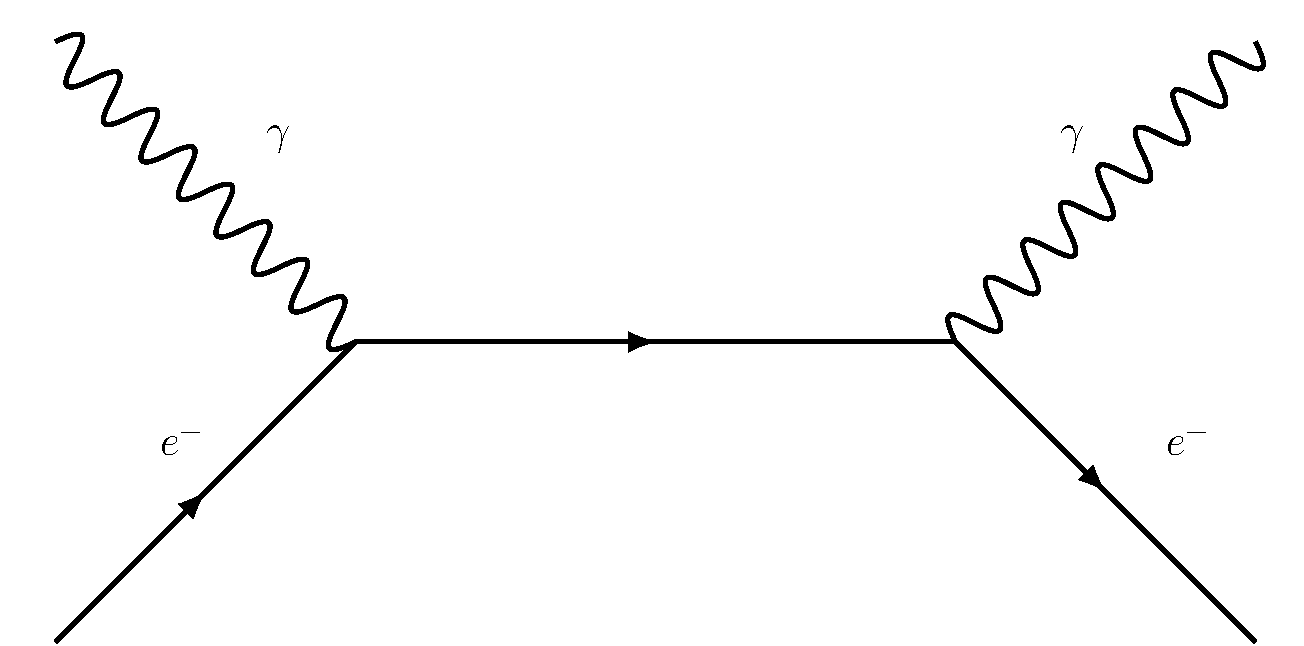
\includegraphics[width=0.9\textwidth]{bilder/compton.pdf}
    \caption{Compton-Effekt. \cite{feynman}}
\end{minipage}
\end{figure}


\begin{equation*}
    \increment \lambda = \frac{h}{m_e c} (1 - \text{cos}(\theta)),
\end{equation*}
wobei $\theta$ den Winkel zwischen ein- und ausfallendem Photon darstellt. 
Wichtig ist, dass durch diesen Effekt neue Phänomene entstehen. Zum einen wird hier das Photon nicht vollständig aufgenommen, sondern nur um einen Energiebruchteil verringert und in eine Richtung $\theta$ gestreut. 
Dies wird sich auch durch eine erhöhte Zählrate niedriger Energien beim Einsetzen möglicher Streuobjekte in den Strahlengang zeigen. Die Winkelverteilungen und Häufigkeiten lassen sich über den Klein-Nishina-Wirkungsquerschnitt ermitteln. 
In dem Energiebereich der Gammastrahlung kommt es bereits vermehrt zum Comptoneffekt, deshalb ist dieser in dem Versuch ein auschlaggebender Prozess.
\subsubsection{Paarbildung}
\begin{figure}
    \begin{minipage}{0.5\textwidth}
        Bei der Paarbildung kommt es zum spontanen Zerfall eines Photons in ein Elektron-Positron-Paar. Es kann gezeigt werden, dass dieser Zerfall nur in Anwesenheit weiterer Teilchen oder Feldern vorkommt. Dies liegt an der nötigen
        Impulserhaltung in allen Energiebereichen. Die minimal nötige Energie des Photons zur Erzeugung eines Elektron-Positron Paars beträgt also der doppelten Elektronenruhemasse und somit $E = \SI{1.022}{\mega\electronvolt}$. Bei genau dieser
        Energie besitzen die Teilchen allerdings keine überschüssige Energie in Form von kinetischer Energie und somit können sie den vorhanden Impuls des Photons nicht kompensieren.
    \end{minipage}
    \begin{minipage}{0.5\textwidth}
        \centering
        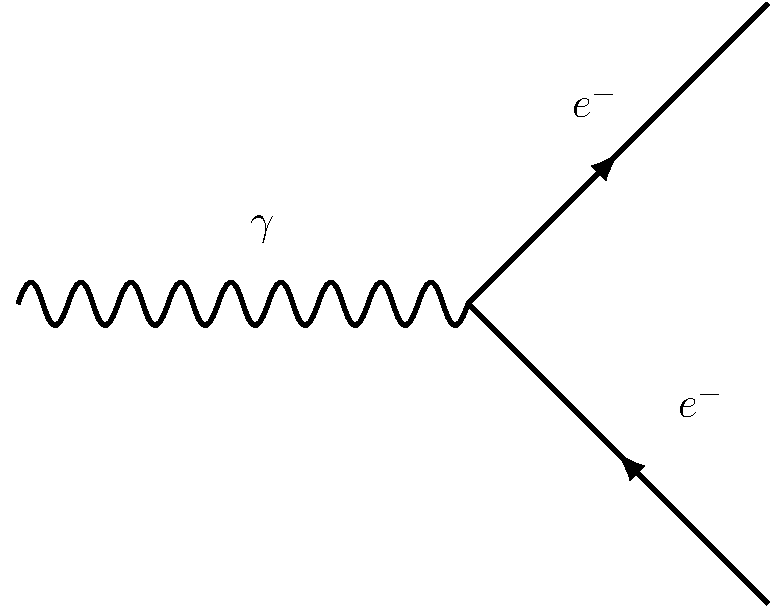
\includegraphics[width=0.9\textwidth]{bilder/paarbildung.pdf}
        \caption{Paarbildung. \cite{feynman}}
        \label{fig:lol1}
    \end{minipage}
    \end{figure}

Eine Abbildung des Prozesses ist in Darstellung \ref{fig:lol1} in Form eines
Feynman-Diagrams gezeigt. Da in diesem Versuch allerdings nur Gammastrahlung unter $E = \SI{1.022}{\mega\electronvolt}$ verwendet wird, ist der Paarbildungseffekt jedoch ausgeschlossen.
\subsection{Tomographie}
Unter der Tomographie versteht sich ein bildgebendes Verfahren, welches ein Gesamtbild aus einzelnen Schnittbildern konstruieren kann. Gemessen wird hierbei
lediglich eine Intensitätsveränderung vor- und hinter dem abzubildendem System. 
Bei dem bekannten Röntgenbild, wird die Intensitätsschwächung ins Zweidimensionale projeziert, während bei der CT (Computertomographie) ein dreidimensionales Bild aus vielen Projektionen erstellt wird. 
In unserem Fall wird lediglich eine Ebene eines Materialblocks auf ihren Inhalt untersucht. Dieser lässt sich dabei aus der Messung einzelner Intensitätsschwächungen rekonstruieren. 
Hierbei werden nun die einzelnen Wirkungsquerschnitte der Wechselwirkungsprozesse interessant.
\subsection{Absorptionskoeffizienten}
Zur Beschreibung des Intensitätsverlustes von Strahlung durch ein Medium wird das Lambert-Beersche Gesetz verwendet. Im Allgemeinen sagt dies lediglich, dass
\begin{equation*}
\text{d}I \propto -I \text{d}x
\end{equation*}
gilt, also das die Intensitätsabnahme proportional zur vorhandenen Intensität und Schichtdicke ist. Diese Differentialgleichung kann gelöst werden und da die Proportionalitätskonstante von dem Material abhängt, folgt
\begin{equation}
    \label{eqn:ayoo}
I(x) = I_0 \text{exp}\left(- \sum_{i}^{} \mu_i x_i \right).
\end{equation}
Die Absorptionskoeffizienten $\mu$ besitzen die Einheit $[\SI{1}{\per\centi\meter}]$ und sie lassen sich für jedes Material und die Photonenenergien aus den Wirkungsquerschnitten $\tilde{\sigma}$ bestimmen. Die beiden wichtigen Prozesse sind der Photoeffekt und Compton Effekt,
also lässt sich ein Gesamterwirkungsquerschnitt als Summe dieser beiden annehmen. Allgemein gilt die Umrechnung von Wirkungsquerschnitt zu Absorptionskoeffizienten wie folgt \cite{hier}
\begin{equation*}
\mu = \tilde{\sigma} \rho \frac{N_\text{A}}{M_{\text{mol}}}.
\end{equation*}
In der Literatur sind die Wirkungsquerschnitte $\sigma$ oft bereits in der Einheit $[\SI{}{\centi\meter\squared\per\gram}]$ angegeben wodurch sich das Verhältnis zu 
\begin{equation*}
\mu = \sigma \rho
\end{equation*}
vereinfacht. In der Tabelle \ref{tab:2} sind die Wirkungsquerschnitte für verschiedene Materialen \cite{wqs} und die errechneten Absorptionskoeffizienten eingetragen. 
\subsection{Bestimmung der Absorptionskoeffizienten}
Durch Logarithmieren und Umformen der Gleichung \eqref{eqn:ayoo} folgt
\begin{equation}
    \label{eqn:hierlol}
\sum_{i}^{} \mu_i x_i = \text{ln}\left(\frac{I_0}{I}\right).
\end{equation}
Diese Gleichung nimmt also die Gestalt eines Skalarproduktes an. Wichtig ist hier, dass es sobald mehr als nur ein Faktor $\mu$ betrachtet wird keine eindeutige Lösbarkeit garantiert ist. Mehrere Parameter lassen sich anhand einer Bedingung
nicht eindeutig bestimmen. Im Allgemeinen gilt, dass mindestens gleich viele Bedingungen wie Parameter vorliegen müssen. Bei einem Würfel mit Neun unbekannten Absorptionskoeffizienten kann dies anhand einer Matrixgleichung aufgeschrieben werden.
Dabei können die Richtungen $x_i$ gemischt werden und es gilt
\begin{equation*}
A \vec{\mu} = \vec{I}.
\end{equation*}
Es handelt sich also um ein lineares inhomogenes Gleichungssystem, wobei die Dimension von $\vec{\mu}$ festgelegt ist. Eine nichttriviale Lösung liegt vor, wenn die Matrix $A$ regulär ist. Wenn sie regulär und quadratisch ist, existiert
eine Inverse Matrix und somit folgt
\begin{equation*}
\vec{\mu} = A^{-1}\vec{I}.
\end{equation*}
Wird nun aber eine Messreihe mit mehr als Neun Messungen konstruiert, so muss die Matrix $A$ zunächst mit seiner Transponierten Matrix $A^{\text{T}}$ multipliziert werden, damit sie quadratisch und somit invertierbar ist. 
Dies lässt sich schreiben als 
\begin{equation*}
\vec{\mu} = (A^{\text{T}}A)^{-1} A^{\text{T}} \vec{I}.
\end{equation*}
Der zu untersuchende Block hat die folgende Auslegung.
\begin{table}
    \centering
    \caption*{} 
    \label{tab:3}
    \begin{tabular}{c | c | c}
        $\mu_1$ & $\mu_2$ & $\mu_3$ \\
        \midrule
        $\mu_4$ & $\mu_5$ & $\mu_6$  \\
        \midrule
        $\mu_7$ & $\mu_8$ & $\mu_9$  \\
    \end{tabular}
\end{table}
\begin{flushleft}
Für die Bestimmung aller Absorptionskonstanten wird die Matrix 
\end{flushleft}
\begin{equation}
    \label{eqn:lul}
A = 
\begin{pmatrix}
    1 & 1 & 1 & 0 & 0 & 0 & 0 & 0 & 0 \\
    0 & 0 & 0 & 1 & 1 & 1 & 0 & 0 & 0 \\
    0 & 0 & 0 & 0 & 0 & 0 & 1 & 1 & 1 \\
    0 & \sqrt{2} & 0 & 0 & 0 & \sqrt{2} & 0 & 0 & 0 \\
    \sqrt{2} & 0 & 0 & 0 & \sqrt{2} & 0 & 0 & 0 & \sqrt{2} \\
    0 & 0 & 0 & \sqrt{2} & 0 & 0 & 0 & \sqrt{2} & 0 \\
    0 & 0 & 1 & 0 & 0 & 1 & 0 & 0 & 1 \\
    0 & 1 & 0 & 0 & 1 & 0 & 0 & 1 & 0 \\
    1 & 0 & 0 & 1 & 0 & 0 & 1 & 0 & 0 \\
    0 & 0 & 0 & 0 & 0 & \sqrt{2} & 0 & \sqrt{2} & 0 \\
    0 & 0 & \sqrt{2} & 0 & \sqrt{2} & 0 & \sqrt{2} & 0 & 0 \\
    0 & \sqrt{2} & 0 & \sqrt{2} & 0 & 0 & 0 & 0 & 0 \\
\end{pmatrix}
\end{equation}
\begin{flushleft}
gewählt. Sie ist mit der Dimension $12 \times 9$ überbestimmt und die einzelnen Messrichtungen sind festgelegt.
\end{flushleft}